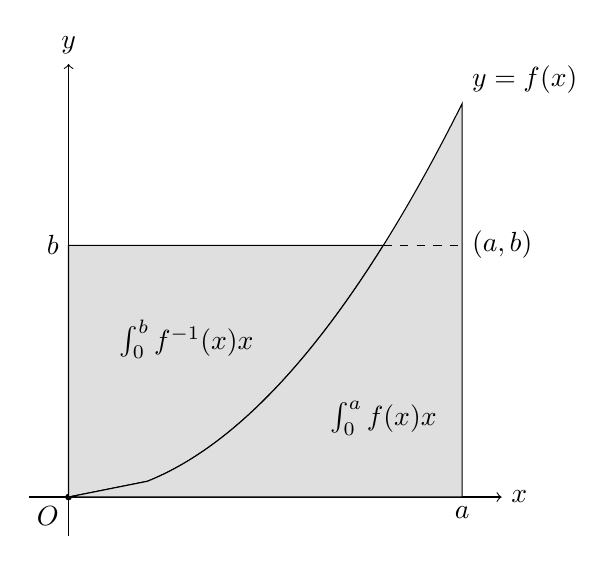
\begin{tikzpicture}
    \draw[->] (-0.5, 0) -- (5.5, 0) node[right] {\(x\)};
    \draw[->] (0, -0.5) -- (0, 5.5) node[above] {\(y\)};
    \filldraw (0, 0) circle (1pt) node[below left] {\(O\)};

    \draw[fill=gray!25] plot[smooth, samples=200, domain=1:4] (\x, \x^2 / 5) -| (0,0) -- cycle;
    \node at (1.5, 2) {\(\int_{0}^{b} f^{-1} (x) \Diff x\)};

    \draw[fill=gray!25] plot[smooth, samples=200, domain=1:5] (\x, \x^2 / 5) |- (0,0) -- cycle;
    \node at (4, 1) {\(\int_{0}^{a} f(x) \Diff x\)};

    \node at (5, 5) [above right] {\(y = f(x)\)};
    \node at (5, 0) [below] {\(a\)};
    \node at (0, 16 / 5) [left] {\(b\)};
    \draw[dashed] (4, 16 / 5) -- (5, 16 / 5) node[right] {\((a, b)\)};
\end{tikzpicture}